\begin{problem}{1}  $ $
\begin{enumerate}
\item
We recognize that this is a uniform random variable, so its CDF is:
\[
  F_X(x) =
  \begin{cases}
                                   0 & \text{for $x < 2$} \\
                                   \frac{x-2}{4} & \text{for $2 \le x \le 6$} \\
 1 & \text{for $x>6$}.
  \end{cases}
\]

\item
For a uniform random variable, the expectation value is at the midpoint: $E[X] = 2+[(6-2)]/2 = 4$.


\end{enumerate}
\end{problem}

\begin{problem}{2}  $ $
\begin{enumerate}

\item By normalization, $1 = c \int_0^\infty \exp{(-4x)}dx$, which leads to $c=4$. 

\item
\begin{equation*}  
  F_X(x) = \begin{cases}
                                   0 & \text{for $~x \le 0$} \\
                                   4\int_0^x e^{-4 x^\prime dx^\prime} & \text{for  $x>0$} 
       \end{cases} \quad
= \begin{cases}
                                   0 & \text{for $~x \le 0$} \\
                                   1 - e^{-4 x} & \text{for  $x>0$}.
       \end{cases}
\end{equation*}

\item

\begin{equation*}
P(2 < X < 5) = 4 \int_2^5 e^{-4x}dx = e^{-8}-e^{-20}.
\end{equation*}

\item
To find the expectation value, I use integration by parts:

\begin{align*}
E[X] &= 4\int_0^\infty x e^{-4x}dx \\
& = -\left(x e^{-4x} \right)_0^\infty +\int_0^\infty e^{-4x}dx \\
& = \frac{1}{4},
\end{align*}

where the limits in the first term were evaluated using L'hopital's rule.

\end{enumerate}
\end{problem}

\begin{problem}{3}  $ $
\begin{enumerate}

\item
Using LOTUS:
\begin{align*}
E\left[X^n\left(X^2+\frac{2}{3}\right)\right] &= \int_0^1 x^n\left(x^2+\frac{2}{3}\right)dx \\
& = \frac{1}{3+n}x^{3+n} \Big|_0^1 +\left(\frac{2}{3}\right)\frac{1}{n+1}x^{n+1} \Big|_0^1 \\
& = \frac{1}{3+n}+\left(\frac{2}{3}\right)\frac{1}{n+1}~~\mathrm{for}~n=1, 2, 3, \ldots
\end{align*}

\item
We have already found $E[X]$ and $E[X^2]$ in the first part and thus:
\begin{align*}
Var[X] & = E[X^2]- E[X]^2 \\
& = \frac{1}{3+2}+\left(\frac{2}{3} \right)\frac{1}{2+1}- \left [ \frac{1}{3+1}+\left(\frac{2}{3} \right)\frac{1}{1+1} \right]^2 \\
& = \frac{59}{720}.
\end{align*}
\end{enumerate}
\end{problem}


\begin{problem}{4} $ $
\begin{enumerate}
\item For this problem, we have $R_X = [0, 1]$ and $R_Y = [1/e, 1]$.  Thus in range of $x=$ 0 to 1, the CDF of $Y$ is given by:

\begin{align*}
F_Y(y) & = P(Y \le y) \\
& = P(e^{-X} \le y ) \\
& = P(X \ge -\ln{y} ) \\
& = 1-F_X(-\ln{y} ) \\
& = 1+\ln y,
\end{align*}
where I used the fact that for $x \in [0, 1]$ for a uniform 0, 1 distribution, $F_X(x)=x$.
Therefore:
\[
  F_Y(y) =
  \begin{cases}
                                   0 & \text{for $y<\frac{1}{e}$} \\
                                   1+\ln(y) & \text{for $\frac{1}{e} \le y \le 1$} \\
                                   1 & \text{for $y>1$}.
  \end{cases}
\]

\item
\[
  f_Y(y) = \frac{ d F_Y}{dy}=
  \begin{cases}
                                   0 & \text{for $y<\frac{1}{e}$} \\
                                   \frac{1}{y} & \text{for $\frac{1}{e} \le x \le 1$} \\
                                   0 & \text{for $x>1$}
  \end{cases}
\]

\item

\begin{equation*}
E[Y] = \int_{1/e}^1 y \frac{1}{y} dy = 1-\frac{1}{e}
\end{equation*}

\end{enumerate}

\end{problem}


\begin{problem}{5} $ $

\begin{enumerate}

\item The range of $X$ and $Y$ are $R_X = (0, 2]$ and $R_Y = (0, 4]$, so that for $y \in R_Y$, we have

\begin{align*}
F_Y(y) &= P(Y \le y)\\
& = P(X^2 \le y) \\
& = P(0  <X < \sqrt{y}) \\
& = \int_0^{\sqrt{y}} \frac{5}{32}x^4 dx \\
& = \frac{1}{32}y^{5/2},
\end{align*} 
and therefore:
\[
  F_Y(y) =
  \begin{cases}
                                   0 & \text{for $y \le 0$} \\
                                   \frac{1}{32}y^{5/2} & \text{for $0<y \le 4$} \\
                                   1 & \text{for $y>4$}.
  \end{cases}
\]

\item 
\[
  f_Y(y) = \frac{ d F_Y}{dy}=
  \begin{cases}
                                   0 & \text{for $y \le 0$} \\
                                  \frac{5}{64}y^{3/2} & \text{for $0<y \le 4$} \\
                                   0 & \text{for $y>4$}
  \end{cases}
\]
 
\item

\begin{equation*}
E[Y] = \frac{5}{64}\int_0^4 y\cdot y^{3/2} \approx 2.9
\end{equation*}
 
\end{enumerate}

\end{problem}





\begin{problem}{6}  We can convert the PDF for $X$ to the PDF for $Y$ using the method of transformations:


\[
  f_Y(y) = f_X\left(\frac{y}{\alpha}\right)\left|\frac{ d (y/\alpha)}{dy}\right|=
  \begin{cases}
                                   \frac{\lambda}{\alpha}e^{-\frac{\lambda}{\alpha} y} & \text{for $y>0$} \\
                                   0 & \text{otherwise} 

  \end{cases},
\]
and since both $\alpha, \lambda>0$, $Y\sim Exp(\lambda/\alpha)$.

\end{problem}

\begin{problem}{7} $ $

\begin{enumerate}
\item  We can prove this relation using integration by parts:

\begin{align*}
E[X^n] &= \int_0^\infty x^n \lambda e^{-\lambda x}dx \\
& = -x^n e^{-\lambda x}\Big|_0^\infty +\frac{n}{\lambda}\int_0^\infty x^{n-1} \lambda e^{\lambda x}dx \\
 & = \frac{n}{\lambda}E[X^{n-1}],
\end{align*}
where the first term evaluated to zero by repeated application of L'Hopital's rule.

\item We can use several properties of the Gamma function to prove this relation:

\begin{align*}
E[X^n] &= \int_0^\infty x^n \lambda e^{-\lambda x}dx \\
&=\frac{\lambda}{\lambda^{n+1}}\Gamma(n+1) \\
& = \frac{n!}{\lambda^n},
\end{align*}
where in the second equality I used the second property of the Gamma function given in the book, and in the third equality I used the fourth property of the Gamma function given in the book.

\end{enumerate}

\end{problem}

\begin{problem}{8} $ $

\begin{enumerate}
\item

\begin{equation*}
P(X>0) = 1- \Phi \left(\frac{0-3}{3} \right) \approx 0.84
\end{equation*}

\item

\begin{equation*}
P(-3<X<8) = \Phi \left(\frac{8-3}{3} \right)- \Phi \left(\frac{-3-3}{3} \right) \approx 0.93
\end{equation*}

\item

\begin{align*}
P(X>5|X>3) &=\frac{P(X>5, X>3)}{P(X>3)} \\
& = \frac{P(X>5)}{P(X>3)} \\
& = \frac{1-\Phi \left(\frac{5-3}{3} \right)}{1-\Phi \left(\frac{3-3}{3} \right)} \\
& \approx 0.50
\end{align*}


\end{enumerate}

\end{problem}

\begin{problem}{9} By Theorem 4.3 in the book, if $X \sim \mathcal N(3, 9)$, and $Y =5-X$, then $Y \sim \mathcal N(-3+5, 9)=\mathcal N(2, 9)$.

\begin{enumerate}
\item 

\begin{equation*}
P(X>2) = 1-\Phi \left(\frac{2-3}{3} \right) \approx 0.63
\end{equation*}

\item

\begin{equation*}
P(-1<Y<3) = \Phi \left(\frac{3-2}{3} \right) -\Phi \left(\frac{-1-2}{3} \right)  \approx 0.47
\end{equation*}

\item

\begin{align*}
P(X>4|Y<2) &=P(X>4|5-X<2) \\
&=\frac{P(X>4, X>3)}{P(X>3)} \\
& = \frac{P(X>4)}{P(X>3)} \\
& = \frac{1-\Phi \left(\frac{4-3}{3} \right)}{1-\Phi \left(\frac{3-3}{3} \right)} \\
& \approx 0.74
\end{align*}


\end{enumerate}

\end{problem}



\begin{problem}{10}  I first note that $R_X = \mathbb R$, and $R_Y=[0, \infty)$.  The range of $X$ can be partitioned into 2 regions, $X \le 0$ and $X>0$ which are strictly decreasing, and increasing respectively, where the corresponding inverse transformation back to $X$ for both of these regions is:
\[
X=
  \begin{cases}
                                   -Y^2 & \text{for $X \le 0$} \\
                                   Y^2 & \text{for $X>0$}.
  \end{cases}
\]
Therefore:
\begin{align*}
f_Y(y) &=f_X(y^2)\left|\frac{d(y^2)}{dy}\right|+f_X(-y^2) \left |\frac{d(-y^2)}{dy}\right |\\
& =\frac{4}{\sqrt{2 \pi}}y e^{-\frac{y^4}{2}} ~~~ \mathrm{for}~ y \ge 0,
\end{align*}
which, as a sanity check, I made sure analytically integrates to unity over the range 0 to infinity.



\end{problem}


\begin{problem}{11} $ $

\begin{enumerate}
\item

\begin{equation*}
P(X>2)  = 2 \int_2^{\infty}e^{-2 x} = e^{-4}
\end{equation*}

\item I calculate $E[Y]$ using LOTUS:

\begin{align*}
E[Y] &= \int_0^\infty (2+3x)2 e^{-2x}dx \\
 & = 2\int_0^\infty 2 e^{-2x}dx+3\int_0^\infty 2x e^{-2x}dx \\
 & = 2+3E[X]\\
 &=2+\frac{3}{2} \\
 & = \frac{7}{2},
\end{align*}
where I have used the fact that $E[X]$ for $Exp(\lambda)$ is $1/\lambda$ (as computed in the book).
To compute $Var[Y]$, I first must compute $E[Y^2]$, which I do using LOTUS:

\begin{align*}
E[Y^2] &= \int_0^\infty (2+3x)^22 e^{-2x}dx \\
 & = 4\int_0^\infty 2 e^{-2x}dx+12\int_0^\infty 2x e^{-2x}dx+9\int_0^\infty 2x^2 e^{-2x}dx \\
 & = 4+12E[X]+9E[X^2]\\
 &=4+\frac{12}{2}+\frac{9 \cdot 2}{4} \\
 & = \frac{29}{2},
\end{align*}
where I have used the fact that $E[X^2]$ for $Exp(\lambda)$ is $2/(\lambda^2)$ (as computed in the book).  Finally, the variance is:

\begin{equation*}
Var[Y] = E[Y^2]-E[Y]^2 = \frac{9}{4}.
\end{equation*}

\item

\begin{align*}
P(X>2|Y<11) &=P(X>2|2+3X<11) \\
&=P(X>2|X<3) \\
&=\frac{P(2<X<3)}{P(X<3)} \\
& = \frac{2 \int_2^3 e^{-2x}dx}{2 \int_0^3 e^{-2x}dx} \\
& = \frac{e^{2}-1}{e^{6}-1}\\
& \approx 1.6 \times 10^{-2}
\end{align*}


\end{enumerate}



\end{problem}



\begin{problem}{12} The equations defining the median for a continuous variable, $P(X<m) =1/2$ and $P(X \ge m) =1/2$,  are actually equivalent.  That is, $P(X<m) =1/2 \Leftrightarrow  P(X \ge m)=1/2$ (which can easily be verified), so we can use whichever is convenient.  Since we know the CDFs for the desired distributions, so using the condition that $P(X<m) =1/2$ will be most convenient.

\begin{enumerate}
\item  The CDF for the $Unif(a, b)$ is:

\[
  P(X < x) =
  \begin{cases}
                                   0 & \text{for $x < a$} \\
                                  \frac{x-a}{b-a} & \text{for $a\le x \le b$} \\
                                   1 & \text{for $x > b$},
  \end{cases}
\]
where I have ignored the equality in the argument of $P$, since $P(X = x)=0$ for a continuous random variable.  Setting this equation equal to $1/2$ and solving for $m$, I find:
\begin{equation*}
m = \frac{b+a}{2},
\end{equation*}
which is the mean of the uniform distribution, which was expected since the uniform distribution is symmetric about its mean.

\item The CDF for the $Exp(\lambda)$ is:

\[
P(Y<y) = 
  \begin{cases}
                                   0 & \text{for $y < 0$} \\
                                   1-e^{-\lambda y} & \text{for $y \ge 0$},
  \end{cases}
\]
where again, I have ignored the equality in the argument of $P$, since $P(Y = y)=0$.  Thus we see that $1/2 = 1- \exp{(-\lambda m)} \implies m = \ln{2}/\lambda$.

\item For the $\mathcal N(\mu, \sigma^2)$, 

\begin{align*}
P(W < m) &= P(W \le m) \\
& = \Phi \left (\frac{m-\mu}{\sigma} \right) \\
& = \frac{1}{2}.
\end{align*}
Since the standard normal is symmetric about 0, this implies that $\Phi(0) = 1/2$, and therefore $(m-\mu)/\sigma = 0$, and thus $m=\mu$.  Since we knew that a Gaussian is symmetric about its mean, this is what we expected.


\end{enumerate}

\end{problem}


\begin{problem}{13} $ $
\begin{enumerate}
\item See Fig.~\ref{fig:prob_13} for a plot of the CDF.  $X$ is a mixed random variable because there is a jump in the CDF at $x=1/4$ (indicating a probability ``point mass" at 1/4 of $P(X=1/4)=1/2$) and the CDF does not exhibit the staircase shape associated with only discrete random variables.

	\begin{figure}[t]
	\centering
      		 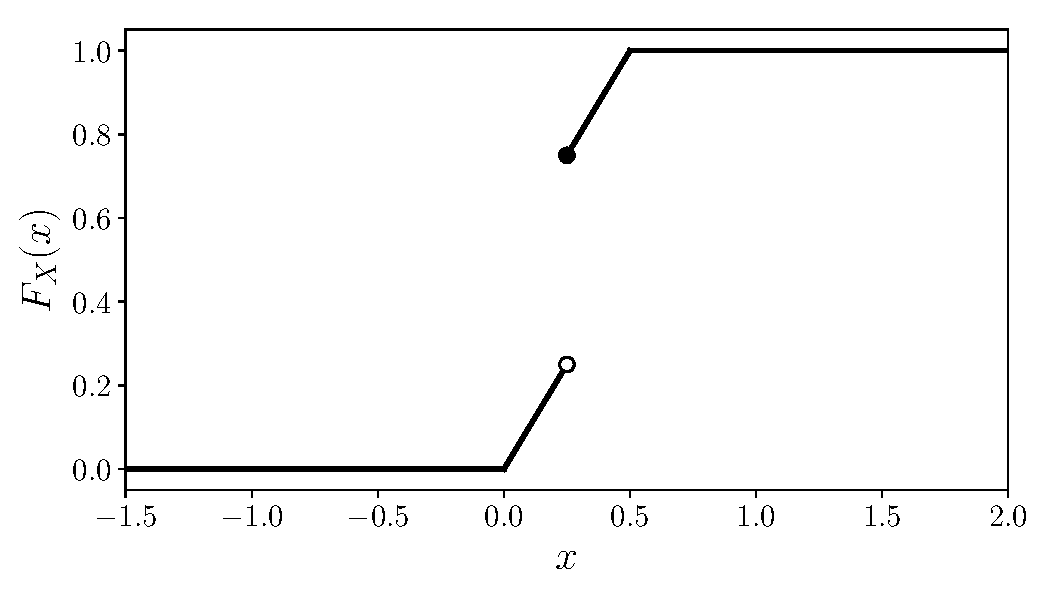
\includegraphics[totalheight=6cm]{chpt4/prob13.pdf}
  			  \caption{CDF for Problem 13}
    			   \label{fig:prob_13}
	\end{figure}

\item
\begin{align*}
P\left(X \le \frac{1}{3}\right) &= F_X\left(\frac{1}{3}\right) \\
&= \frac{1}{3} +\frac{1}{2}  \\
&= \frac{5}{6}
\end{align*}

\item 
\begin{align*}
P\left(X \ge \frac{1}{4}\right) &= 1 - P\left(X<\frac{1}{4}\right) \\
& = 1-\left[P\left(X \le \frac{1}{4}\right)-P\left(X=\frac{1}{4}\right)\right] \\
& = 1-\left[F_X\left(\frac{1}{4}\right)-P\left(X=\frac{1}{4}\right)\right] \\
& = 1-\left(\frac{1}{4}+\frac{1}{2}-\frac{1}{2}\right) \\
& = \frac{3}{4}
\end{align*}

\item

The CDFs for both the discrete and continuous contributions can be written piece-wise as:
\[
D(x) = 
  \begin{cases}
                                   0 & \text{for $x < \frac{1}{4}$} \\
                                   \frac{1}{2}& \text{for $x \ge \frac{1}{4}$},
  \end{cases}
\]
and
\[
C(x) = 
  \begin{cases}
                                   0 & \text{for $x < 0$} \\
                                   x & \text{for $\frac{1}{2} \le x \le \frac{1}{2}$} \\
                                   \frac{1}{2}& \text{for $x>\frac{1}{2}$}.
  \end{cases}
\]
These functions can be re-written using the unit step function:
\begin{equation*}
D(x) = \frac{1}{2}u\left(x-\frac{1}{4}\right),
\end{equation*}
and
\begin{equation*}
C(x) = xu(x) -  xu\left(x-\frac{1}{2}\right)+\frac{1}{2}u\left(x-\frac{1}{2}\right),
\end{equation*}
where, in $C(x)$, I have started subtracting off the linear equation at $x=1/2$, and adding a constant 1/2 at $x=1/2$ so as to keep the function flat at 1/2 after $x=1/2$.

\item
Since $C(x)$ increases linearly from 0 to 1/2, and has total probability mass 1/2, we expect $c(x)$ to be uniform with height 1 over the range 0 to 1/2.  Differentiating $C(x)$

\begin{align*}
c(x) & = \frac{d}{dx}C(x) \\
& = u(x) +x \frac{du(x)}{dx}-u\left(x-\frac{1}{2}\right)-x \frac{d}{dx}u\left(x-\frac{1}{2}\right)+\frac{1}{2}\frac{d}{dx}u\left(x-\frac{1}{2}\right) \\
& = u(x)+x\delta(x) - u \left (x-\frac{1}{2}\right)-x\delta \left(x-\frac{1}{2}\right)+\frac{1}{2}\delta \left(x-\frac{1}{2}\right) \\
& = u(x) -u\left(x-\frac{1}{2}\right),
\end{align*}
which is exactly what we had anticipated.  Here I used the fact that when $x \ne 1/2$, $x\delta(x-1/2)$ and $(-1/2)\delta(x-1/2)$ equal 0, while for for $x =1/2$, $(-1/2) \delta(x-1/2) = (-1/2)\delta(0)$ and $x \delta(x-1/2) = (1/2)\delta(0)$.  Also, in either case, $x \delta(x) = 0$.

\item

\begin{align*}
E[X] &= \int_{-\infty}^{\infty}x c(x) dx+\sum_{k}x_k a_k \\
& = \int_0^{1/2}x dx+\frac{1}{4}P\left(X=\frac{1}{4}\right) \\
& = \frac{1}{2}x^2\Big|_0^{1/2} dx+\frac{1}{4}\cdot \frac{1}{2} \\
& = \frac{1}{4}
\end{align*}

\end{enumerate}


\end{problem}


\begin{problem}{14}$ $


\begin{enumerate}
\item The generalized PDF of X is:
\begin{align*}
f_X(x) &= \frac{d}{dx}F_X(x) \\
& =   \frac{d}{dx}D(x)+\frac{d}{dx}C(x) \\
& = \frac{1}{2}\delta \left(x-\frac{1}{4}\right)+c(x) \\
& =  \frac{1}{2}\delta \left(x-\frac{1}{4}\right)+\left[u(x)-u\left(x-\frac{1}{2}\right)\right],
\end{align*}
where $c(x)$ was found in the previous problem.

\item
\begin{align*}
E[X] &= \frac{1}{2}\int_{-\infty}^{\infty}x\delta \left(x-\frac{1}{4}\right)dx + \int_{-\infty}^{\infty}xu(x)dx-\int_{-\infty}^{\infty}xu\left(x-\frac{1}{2}\right)dx \\
&= \frac{1}{2}\int_{-\infty}^{\infty}x\delta \left(x-\frac{1}{4}\right)dx + \int_0^{1/2}x dx\\
& = \frac{1}{2}\cdot\frac{1}{4}+\frac{1}{8} \\
& = \frac{1}{4}
\end{align*}


\item
\begin{align*}
E[X^2]&=\frac{1}{2}\int_{-\infty}^{\infty}x^2\delta \left(x-\frac{1}{4}\right)dx + \int_{0}^{1/2}x^2dx \\
& = \frac{1}{2} \left(\frac{1}{4} \right)^2+\frac{1}{3}x^3\Big|_0^{1/2} \\
& = \frac{7}{96}
\end{align*}
$\implies$
\begin{align*}
Var[X]&=E[X^2] - E[X]^2 \\
& =  \frac{7}{96} - \left(\frac{1}{4}\right)^2 \\
& = \frac{1}{96}
\end{align*}



\end{enumerate}

\end{problem}

\begin{problem}{15} $ $

\begin{enumerate}
\item

From the form of the given generalized PDF, it is clear that there are 2 probability point masses at $x=1$ and $x=-2$ (with $P(X=1)=1/6$ and $P(X=-2)=1/3$), as well as a continuous random variable contribution from a Gaussian PDF.  Since the continuous PDF contributes 0 probability at specific points, $P(X=1)=1/6$ and $P(X=-2)=1/3$.


\item

\begin{align*}
P(X \ge 1)& = \int_1^{\infty} \left [ \frac{1}{3}\delta(x+2) +\frac{1}{6}\delta(x-1)+\frac{1}{2}\frac{1}{\sqrt{2 \pi}}e^{-\frac{x^2}{2}} \right] dx \\
& = \frac{1}{6}+\frac{1}{2}\int_{1}^\infty  \frac{1}{\sqrt{2 \pi}}e^{-\frac{x^2}{2}}dx \\
& = \frac{1}{6}+\frac{1}{2} \left [ 1-\Phi(1) \right] \\
& \approx 0.25
\end{align*}

\item

\begin{align*}
P(X=1|X \ge 1) &= \frac{P(X=1, X \ge 1)}{P(X \ge 1)} \\
&= \frac{P(X=1)}{P(X \ge 1)} \\
&= \frac{\frac{1}{6}}{ \frac{1}{6}+\frac{1}{2} \left [ 1-\Phi(1) \right]} \\
& \approx 0.68
\end{align*}

\item We can calculate $E[X]$ by explicitly integrating over the generalized PDF:
\begin{align*}
E[X] & = \int_{-\infty}^{\infty} x \left [ \frac{1}{3}\delta(x+2) +\frac{1}{6}\delta(x-1)+\frac{1}{2}\frac{1}{\sqrt{2 \pi}}e^{-\frac{x^2}{2}} \right] dx\\
& = \frac{1}{3}(-2)+\frac{1}{6}(1)+\frac{1}{2}\int_{-\infty}^{\infty} x \frac{1}{\sqrt{2 \pi}}e^{-\frac{x^2}{2}} dx \\
& = \frac{-2}{3} +\frac{1}{6}+\frac{1}{2}\cdot 0 \\
& = -\frac{1}{2},
\end{align*}
where the integral in the second line is equal to zero, since this is just the mean of a standard normal distribution.

We can also calculate $E[X^2]$ by explicitly integrating over the generalized PDF:
\begin{align*}
E[X^2] & = \int_{-\infty}^{\infty} x^2 \left [ \frac{1}{3}\delta(x+2) +\frac{1}{6}\delta(x-1)+\frac{1}{2}\frac{1}{\sqrt{2 \pi}}e^{-\frac{x^2}{2}} \right] dx\\
& = \frac{1}{3}(4)+\frac{1}{6}(1)+\frac{1}{2}\int_{-\infty}^{\infty} x^2 \frac{1}{\sqrt{2 \pi}}e^{-\frac{x^2}{2}} dx \\
& = \frac{4}{3} +\frac{1}{6}+\frac{1}{2}(1) \\
& =2,
\end{align*}
where the integral in the second line is equal to 1, since this is just the variance of a standard normal distribution.

Thus:
\begin{align*}
Var[X]&=E[X^2] - E[X]^2 \\
& = 2 - \left(-\frac{1}{2}\right)^2 \\
& = \frac{7}{4}.
\end{align*}

\end{enumerate}



\end{problem}


\begin{problem}{16} $ $

\begin{enumerate}
\item Let $D$ denote the event that the device is defective, and let $P(D) = p_d = 0.02$.  By the law of total probability, we have:

\begin{align*}
F_X(x) &= P(X \le x) \\
&= P(X \le x|D)P(D)+ P(X \le x|D^c)P(D^c)\\
&= u(x)p_d+(1-e^{-\lambda x})(1-p_d)u(x).
\end{align*}

By differentiating, we can find the generalized PDF:
\begin{align*}
f_X(x) &= \frac{d}{dx} F_X(x) \\
&= p_d \delta(x) +(1-p_d)\left[(1-e^{-\lambda x}) \delta(x) +u(x) \lambda e^{-\lambda x} \right] \\
& =p_d \delta(x) +(1-p_d)u(x) \lambda e^{-\lambda x},
\end{align*}
where I have used the fact that at $x \ne 0$, $\delta(x)=0$, and at $x=0$, $(1-\exp{(-\lambda x)})=0$, so that the term, $(1-e^{-\lambda x}) \delta(x)$ is 0 for all $x$.  We also could have written this PDF down immediately by realizing that there is a probability point mass at $x=0$ with total probability $0.02$, and there is a continuous probability contribution from the exponential distribution which must integrate to $1-0.02=0.98$.

\item

\begin{align*}
P(X \ge 1) &= \int_1^{\infty}\left [p_d \delta(x)+(1-p_d)u(x)\lambda e^{-\lambda x} \right] dx \\
& = (1-p_d)\int_1^{\infty}\lambda e^{-\lambda x}dx \\
& = (1-p_d)e^{-\lambda} \\
& = (0.98)e^{-2} \\
& \approx 0.133
\end{align*}

\item
\begin{align*}
P(X >2| X \ge 1) &= \frac{P(X >2,X\ge 1) }{P(X \ge 1) }  \\
&= \frac{P(X >2) }{P(X \ge 1) } \\
&= \frac{\int_2^{\infty}e^{-\lambda x}dx}{\int_1^{\infty}e^{-\lambda x}dx} \\
& = e^{-\lambda} \\
& = e^{-2} \\
& \approx 0.135
\end{align*}

\item
The expectation value of $X$ is:
\begin{align*}
E[X] &= \int_{-\infty}^{\infty}x\left [p_d \delta(x)+(1-p_d)u(x)\lambda e^{-\lambda x} \right] dx \\
&= (1-p_d)\int_0^{\infty}x\lambda e^{-\lambda x}dx \\
&= (1-p_d)\frac{1}{\lambda} \\
&= (0.98)\frac{1}{2} \\
&=0.49,
\end{align*}
where I have used the fact that $E[X] = 1/\lambda$ for an exponential distribution.

The expectation value of $X^2$ is:
\begin{align*}
E[X^2] &= \int_0^{\infty}x^2\left [p_d \delta(x)+(1-p_d)u(x)\lambda e^{-\lambda x} \right] dx \\
&= (1-p_d)\int_0^{\infty}x^2\lambda e^{-\lambda x}dx \\
&= (1-p_d)\frac{2}{\lambda^2} \\
&= (0.98)\frac{1}{2} \\
&=0.49,
\end{align*}
where I have used the fact that $E[X^2] = 2/\lambda^2$ for an exponential distribution.  Therefore, the variance is:
\begin{align*}
Var[X]&=0.49 - 0.49^2 \\
& \approx 0.25.
\end{align*}
\end{enumerate}
\end{problem}

\begin{problem}{17} $ $

\begin{enumerate}
\item
We realize that for $Lap(0, 1)$, $f_X(x)$ is an even function, while $x$ is an odd function and therefore $E[X]=0$.  Also, 
\begin{align*}
E[X^2] = 2\int_0^{\infty}x^2\frac{1}{2}e^{-x}dx
&=2,
\end{align*}
where I have used the fact that since we are integrating an even function times an even function we need only integrate from $0$ to $\infty$ and multiply by 2.  I have also used the fact that the integrand is $E[X^2]$ of an $Exp(1)$ distribution, and we know this integral evaluates to $2/\lambda^2$.  Therefore $Var[X] = 2$.

\item We can solve for $f_Y(y)$ using the method of transformations:

\begin{align*}  
  f_Y(y) &= f_X\left(\frac{y-\mu}{b} \right)\left | \frac{d}{dy}\left(\frac{y-\mu}{b} \right) \right| \\
&=  \begin{cases}
                                   \frac{1}{2}\exp{\left( \frac{y-\mu}{b}\right)}\frac{1}{b} & \text{for $\frac{y-\mu}{b}<0$} \\
                                  \frac{1}{2}\exp{\left[-\left( \frac{y-\mu}{b}\right)\right]}\frac{1}{b}  & \text{for  $\frac{y-\mu}{b}\ge0$} 
       \end{cases} \quad \\
&= \begin{cases}
                                   \frac{1}{2b}\exp{\left( \frac{y-\mu}{b}\right)} & \text{for $y< \mu$} \\
                                  \frac{1}{2b}\exp{\left[-\left( \frac{y-\mu}{b}\right)\right]}  & \text{for  $y\ge \mu$},
       \end{cases}
\end{align*}
which is $Lap(\mu, b)$.

\item
Since
\begin{align*}
E[Y] & = E[bX+\mu] \\
& = bE[X]+\mu \\
& = \mu,
\end{align*}
and
\begin{align*}
E[Y^2] & = E[(bX+\mu)^2] \\
& = b^2E[X^2]+2b \mu E[X]+\mu^2 \\
& = 2b^2 +\mu^2,
\end{align*}
the variance is $Var[Y] = E[Y^2]-E[Y]^2= 2b^2$.

\end{enumerate}
\end{problem}

\begin{problem}{18} We see firstly, that $R_X = \mathbb R$ and $R_Y = [0, \infty)$.  Also note that $Y = |X| = -X$ for $X<0$ and $X$ for $X\ge 0$. I use the method of transformations, breaking $f_X(x)$ into 2 strictly monotonic regions.  Let $f_X^{(1)}(x) = (1/2b)\exp{(x/b)}$ and $f_X^{(2)}(x) = (1/2b)\exp{(-x/b)}$, then:

\begin{align*}
f_Y(y) &= f_X^{(1)}(-y)\left | \frac{dy}{dy} \right|+ f_X^{(2)}(y)\left | \frac{d(-y)}{dy} \right|\\
& = \frac{1}{2b}\exp{\left(-\frac{y}{b} \right)}+\frac{1}{2b}\exp{\left(-\frac{y}{b} \right)} \\
& = \frac{1}{b}\exp{\left(-\frac{y}{b} \right)},
\end{align*}
which is $Exp(1/b)$.

\end{problem}

\begin{problem}{19}$ $
Letting $u \equiv 1+x^2$, the expectation value becomes:

\begin{align*}
E[X] &= \int_{-\infty}^0\frac{1}{\pi}\frac{x}{1+x^2}dx+\int_{0}^\infty \frac{1}{\pi}\frac{x}{1+x^2}dx \\
& = \int_\infty^1 \frac{1}{2 \pi} \frac{du}{u}+\int_1^\infty \frac{1}{2 \pi} \frac{du}{u} \\
& = \frac{1}{2\pi} \ln(1+x^2)\Big|_\infty^1+\frac{1}{2\pi} \ln(1+x^2)\Big|_1^\infty\\
& = -\infty +\infty, 
\end{align*}
which is not well defined.


\begin{align*}
E[X^2]& = \int_{-\infty}^\infty\frac{1}{\pi}\frac{x^2}{1+x^2}dx \\
& =  \frac{2}{\pi}\int_{0}^\infty \frac{x^2}{1+x^2}dx \\
& = \frac{2}{\pi}\left [x -\arctan(x) \right]_0^\infty \\
& = \frac{2}{\pi} \lim_{x \rightarrow \infty}[x -\arctan(x) ] \\
& =\frac{2}{\pi} \lim_{x \rightarrow \infty}x -\frac{2}{\pi} \cdot \frac{\pi}{2} \\
& = \infty
\end{align*}

\end{problem}


\begin{problem}{20}$ $
\begin{enumerate}
\item The expectation value is:
	\begin{align*}
	E[X] &= \frac{1}{\sigma^2}\int_0^\infty x^2e^{-x^2/2\sigma^2}dx \\
	& = \frac{\sqrt{2 \pi}}{2 \sigma}\left[\frac{2}{\sqrt{2 \pi} \sigma}\int_0^\infty x^2e^{-x^2/2\sigma^2}dx\right] \\
	& \frac{\sqrt{2 \pi}}{2 \sigma}\sigma^2 \\
	& = \sigma \sqrt{\frac{\pi}{2}},
	\end{align*}
where I have use the fact that the term in the brackets is the same integral one must compute to find the variance of a $0, \sigma^2$ normal distribution.

\item The integral we must calculate is
	\begin{align*}
	F_X(x) = \int_0^{x} \frac{x^\prime}{\sigma^2} e^{-\frac{{x^\prime}^2}{2 \sigma^2}}dx^\prime,
	\end{align*}
	which can be computed by a simple substitution, $u \equiv {x^\prime}^2/(2\sigma^2)$, so that:
	\begin{align*}
	F_X(x) = \int_0^{\frac{x^2}{2\sigma^2}} e^{-u} du = 1 - e^{-\frac{x^2}{2 \sigma^2}}.
	\end{align*}

\item The range of both $X$ and $Y$ is $[0, \infty)$.  Therefore, for all $y \in [0, \infty)$:


\begin{align*}  
  f_Y(y) &= f_X \left(\frac{y^2}{2 \sigma^2}\right) \left|\frac{d}{dy}\left(\frac{y^2}{2\sigma^2}\right) \right| \\
&= \begin{cases}
                                   \frac{y}{\sigma^2} e^{-\frac{y^2}{2\sigma^2}} & \text{for $y \ge 0$} \\
                                   0 & \text{for  $y<0$},
       \end{cases}
\end{align*}
which is $Rayleigh(\sigma)$.
\end{enumerate}
\end{problem}

\begin{problem}{21}$ $
\begin{enumerate}
\item The CDF is given by:
	\begin{align*}
	F_X(x) &= \alpha x_m^\alpha \int_{x_m}^x {x^\prime}^{-\alpha-1}dx^\prime \\
	& = 1- \left(\frac{x_m}{x} \right)^\alpha
	\end{align*}
for $x\ge x_m$ and $0$ otherwise.
	
\item
	\begin{align*}
P(X>3 x_m|X>2x_m)&=\frac{P(X>3 x_m, X>2x_m)}{P(X>2x_m)} \\
& = \frac{P(X>3 x_m)}{P(X>2x_m)} \\
& = \frac{1- P(X \le 3 x_m)}{1- P(X\le 2x_m)}\\
& = \frac{1- F_X(3x_m)}{1- F_X(2x_m)}\\
& = \frac{1- \left [1-\left(\frac{x_m}{3x_m} \right)^\alpha \right]}{1- \left [1-\left(\frac{x_m}{2x_m} \right)^\alpha \right]}\\
& = \left( \frac{2}{3} \right)^\alpha
	\end{align*}
	
\item The expectation value is:
	\begin{align*}
	E[X] &= \alpha x_m^\alpha \int_{x_m}^\infty x^{-\alpha -1}xdx \\
	&=\frac{\alpha x_m^\alpha}{1-\alpha }\left[ \frac{ x}{x^\alpha}\right]_{x_m}^\infty \\
	& = \frac{\alpha x_m}{\alpha -1},
	\end{align*}
where the $\lim_{x \rightarrow \infty} (x/x^\alpha)$ term evaluates to 0 since $\alpha>2$.  The expectation value of $X^2$ is:
	\begin{align*}
	E[X^2] &= \alpha x_m^\alpha \int_{x_m}^\infty x^{1-\alpha}xdx \\
	& = \frac{\alpha x_m^2}{\alpha -2},
	\end{align*}
where the $\lim_{x \rightarrow \infty} (x^2/x^\alpha)$ term evaluates to 0 since $\alpha>2$.  Thus, the variance is
	\begin{align*}
	Var[X] &= E[X^2]-E[X]^2 \\
	& =  \frac{\alpha x_m^2}{\alpha -2} - \left ( \frac{\alpha x_m}{\alpha -1} \right)^2 \\
	& = \frac{\alpha x_m^2}{(\alpha -1)^2(\alpha -2)}.
	\end{align*}

	\end{enumerate}
\end{problem}



\begin{problem}{22}$ $
\begin{enumerate}

\item

	\begin{align*}
	F_X(x) & = P(X\le x) \\
	& = P(e^{\sigma Z+\mu}\le x) \\
		& = P\left(Z \le \frac{\ln{x}-\mu}{\sigma}\right) \\
		&=\Phi \left (\frac{\ln{x}-\mu}{\sigma} \right)
	\end{align*}
	
\item  I first find the PDF for the log-normal distribution:
		\begin{align*}
	f_X(x) & = \frac{d}{dx} F_X(x) \\
	& = \frac{d}{dx} \Phi \left (\frac{\ln{x}-\mu}{\sigma} \right) \\
		& = \Phi^\prime \left (\frac{\ln{x}-\mu}{\sigma} \right) \frac{1}{x\sigma} \\
		&=f_Z \left (\frac{\ln{x}-\mu}{\sigma} \right) \frac{1}{x\sigma} \\
		& = \frac{1}{x}\frac{1}{\sqrt{2 \pi} \sigma}\exp{\left[-\frac{1}{2} \left(\frac{\ln{x}-\mu}{\sigma} \right)^2\right]},
	\end{align*}
for all $x \in (0, \infty)$.  The expectation value of $X$ is thus
\begin{equation*}
E[X] = \frac{1}{\sqrt{2 \pi} \sigma}\int_0^\infty \exp{\left[-\frac{1}{2} \left(\frac{\ln{x}-\mu}{\sigma} \right)^2\right]},
 \end{equation*}
 which can be simplified with the following substitution:
 \begin{equation*}
u \equiv \ln{x}-\mu,
 \end{equation*}
 $\implies$
  \begin{equation*}
du \equiv \frac{1}{x}dx = e^{-(u+\mu)}dx,
 \end{equation*}
 so that:
 \begin{align*}
E[X] &= \frac{1}{\sqrt{2 \pi} \sigma}\int_{-\infty}^\infty \exp{\left(-\frac{1}{2} \cdot \frac{u^2}{\sigma^2}\right)} \exp{(u+\mu)}du \\
& =  \exp{\left(\mu+\frac{\sigma^2}{2} \right)} \frac{1}{\sqrt{2 \pi} \sigma}\int_{-\infty}^\infty \exp{\left[-\frac{1}{2 \sigma^2} (u-\sigma^2)^2 \right]}du \\
& =\exp{\left(\mu+\frac{\sigma^2}{2} \right)}.
 \end{align*}
 To go from the first equality to the second, I used the ``completing the squares" trick to make the exponent in the form of a Gaussian for easy integration.  In going from the second equality to the third, I used the fact that $1/(\sqrt{2 \pi} \sigma)$ times the integral evaluates to 1 since this is just a $\sigma^2$, $\sigma^2$ Gaussian.
 
 The expectation value of $X^2$ is
\begin{equation*}
E[X^2] = \frac{1}{\sqrt{2 \pi} \sigma}\int_0^\infty x \exp{\left[-\frac{1}{2} \left(\frac{\ln{x}-\mu}{\sigma} \right)^2\right]},
 \end{equation*}
 and we can make the same substitutions, resulting in 
  \begin{align*}
E[X^2] &= \frac{1}{\sqrt{2 \pi} \sigma}\int_{-\infty}^\infty \exp{\left(-\frac{1}{2} \cdot \frac{u^2}{\sigma^2}\right)} \exp{(2u+2 \mu)}du \\
& =  \exp{\left(2 \mu+2\sigma^2 \right)} \frac{1}{\sqrt{2 \pi} \sigma}\int_{-\infty}^\infty \exp{\left[-\frac{1}{2 \sigma^2} (u-2\sigma^2)^2 \right]}du \\
& =\exp{\left(2\mu+2\sigma^2 \right)},
 \end{align*}
 where, again, I used the completing the squares trick, and where the $1/(\sqrt{2 \pi} \sigma)$ times the integral evaluates to 1 since this is just a  $2\sigma^2$, $\sigma^2$  Gaussian.  
 
 Therefore:
 
 	\begin{align*}
	Var[X] &= E[X^2]-E[X]^2 \\
	& =  \exp{(2 \mu +\sigma^2)}\left(\exp{\sigma^2}-1 \right).
	\end{align*}
 

	\end{enumerate}
\end{problem}



\begin{problem}{23}
The expectation value is:
\begin{equation*}
E[Y] = E[X_1+X_2+\ldots+X_n]=nE[X_1] = \frac{n}{\lambda},
\end{equation*}
since the expectation value for an $Exp(\lambda)$ distribution is $1/\lambda$.

Since $X_1, X_2, \ldots ,X_n$ and iid, the variance is linear, and thus:
\begin{equation*}
Var[Y] = Var[X_1+X_2+\ldots+X_n]=nVar[X_1] = \frac{n}{\lambda^2},
\end{equation*}
since the variance for an $Exp(\lambda)$ distribution is $1/\lambda^2$.
\end{problem}


